\section{Instalación del servidor réplica de FreeIPA}\label{sec:instalacion-servidor-replica}

La creación de la máquina virtual destinada a alojar el servidor de réplica se realizó siguiendo el mismo procedimiento empleado para el servidor principal. En consecuencia, se utilizaron las mismas especificaciones de procesamiento, memoria y almacenamiento definidas durante la fase de diseño.

La principal diferencia con respecto a la configuración anterior correspondió a los parámetros de red, ya que fue necesario asignar una dirección \ac{IP} diferente para identificar de manera única el nuevo servidor dentro de la infraestructura. La configuración aplicada a la máquina virtual de la réplica se presenta en la \autoref{fig:configuracion-ip-ipa2}.

\begin{figure}[H]
	\centering
	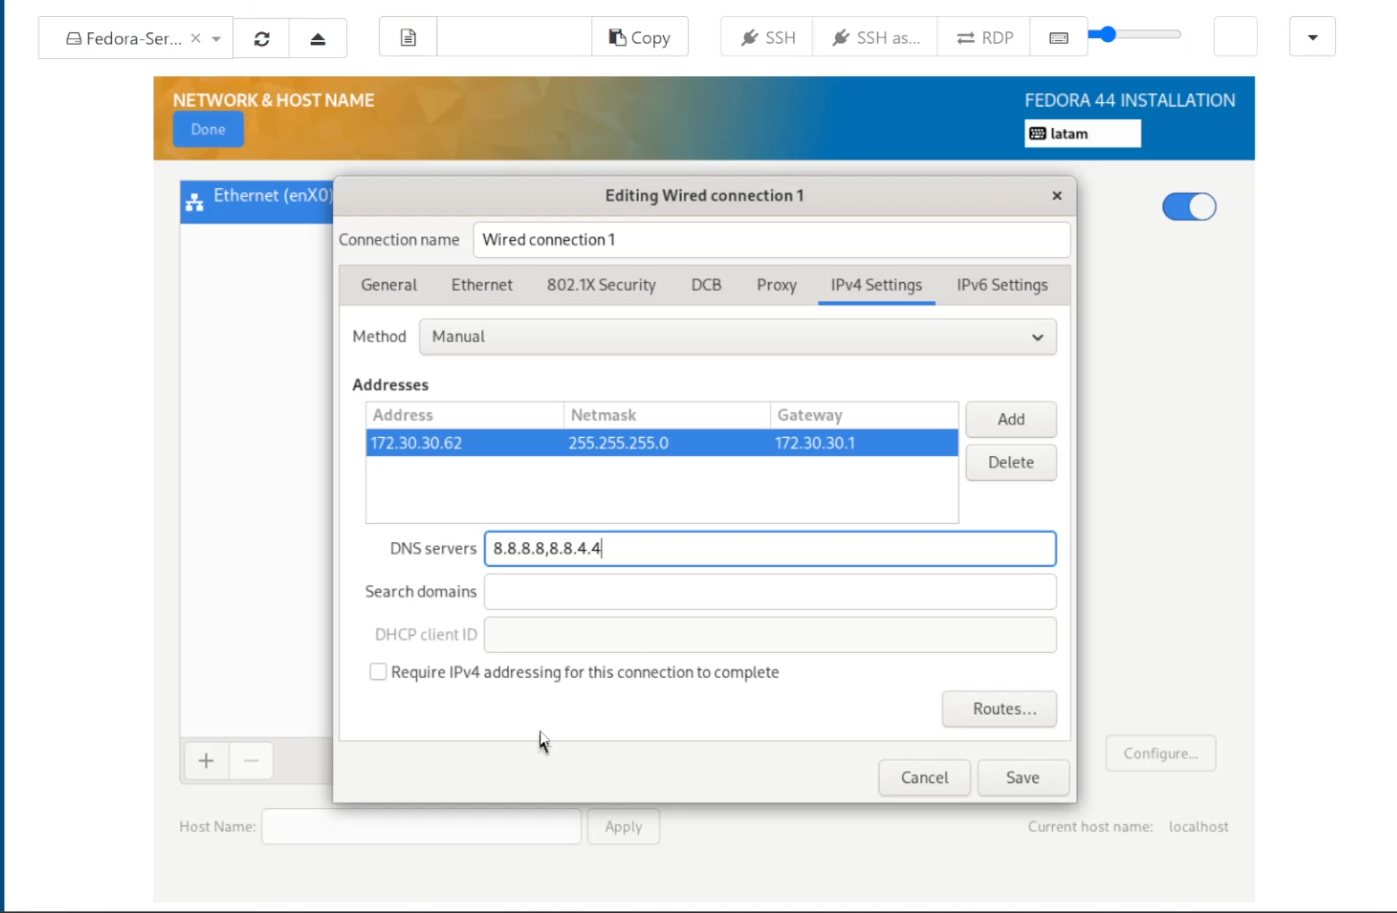
\includegraphics[width=0.8\textwidth]{mainmatter/II-desarrollo-metodologico/implementacion/imagenes/configuracion-ip-ipa2.png}
	\caption{Configuración de red del servidor de réplica}
	\label{fig:configuracion-ip-ipa2}
\end{figure}

Una vez creada la máquina virtual destinada al servidor de réplica y realizada la configuración inicial de la red, se procedió a efectuar las configuraciones previas necesarias para su incorporación a la infraestructura. En esta etapa se empleó el método de promover un cliente recomendado por la documentación oficial de FreeIPA, el cual consiste en transformar un cliente previamente registrado en un servidor de réplica.

Como primer paso, se configuró el nombre de dominio completamente calificado (\ac{FQDN}) del nuevo servidor, con el propósito de garantizar su correcta identificación dentro de la infraestructura. La configuración realizada se muestra en la \autoref{fig:nombre-host-ipa2}.

\begin{figure}[H]
	\centering
	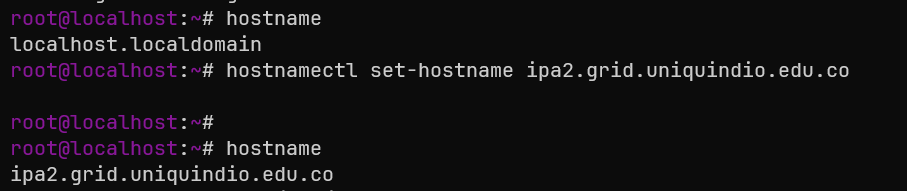
\includegraphics[width=0.8\textwidth]{mainmatter/II-desarrollo-metodologico/implementacion/imagenes/nombre-host-ipa2.png}
	\caption{Configuración del \acs{FQDN} del servidor de réplica}
	\label{fig:nombre-host-ipa2}
\end{figure}

Posteriormente, se habilitaron los servicios correspondientes a \ac{LDAP} y \ac{LDAPS} en el cortafuegos del sistema, con el fin de permitir la comunicación entre los diferentes componentes de la plataforma y garantizar el correcto funcionamiento de los servicios asociados a FreeIPA. En la \autoref{fig:reglas-cortafuegos-ipa2} se presenta la configuración aplicada.

\begin{figure}[H]
	\centering
	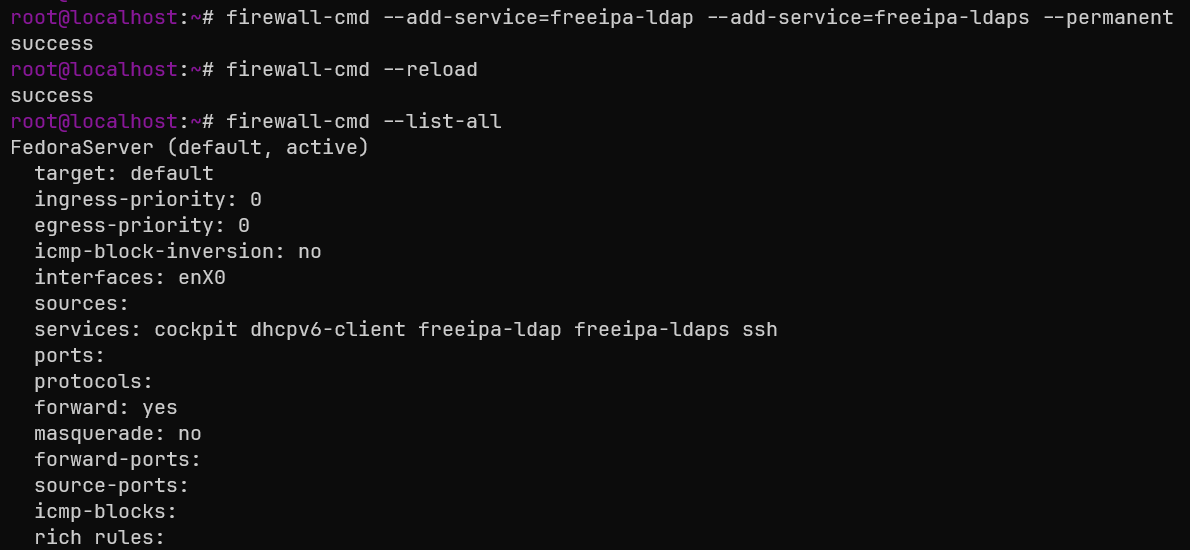
\includegraphics[width=0.8\textwidth]{mainmatter/II-desarrollo-metodologico/implementacion/imagenes/reglas-cortafuegos-ipa2.png}
	\caption{Configuración del cortafuegos del servidor de réplica}
	\label{fig:reglas-cortafuegos-ipa2}
\end{figure}

A continuación, se instaló el paquete freeipa-server, que incorpora las herramientas y dependencias necesarias para la implementación del servidor. En la \autoref{fig:instalacion-paquete-ipa2} se observa el procedimiento realizado.

\begin{figure}[H]
	\centering
	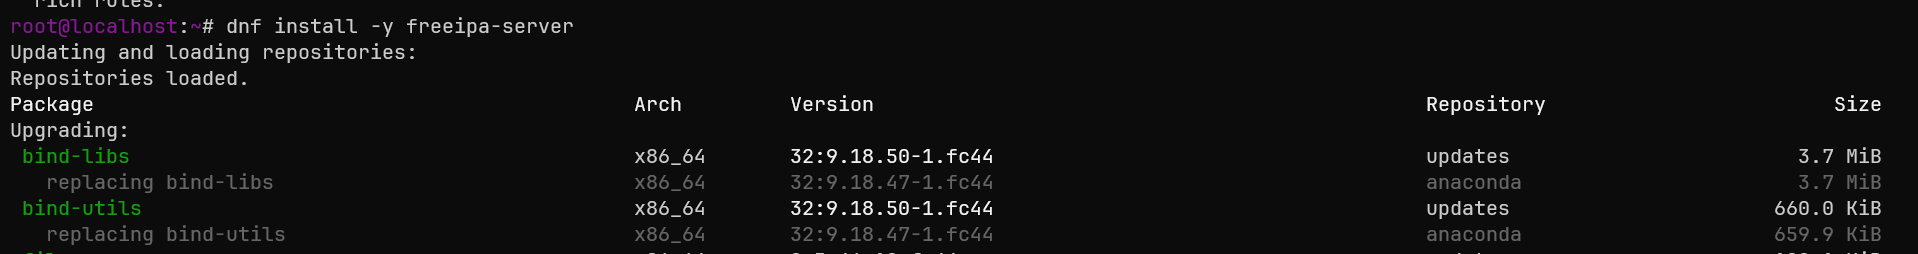
\includegraphics[width=0.8\textwidth]{mainmatter/II-desarrollo-metodologico/implementacion/imagenes/instalacion-paquete-ipa2.png}
	\caption{Instalación del paquete freeipa-server}
	\label{fig:instalacion-paquete-ipa2}
\end{figure}

Una vez completado este proceso, se instaló el cliente de FreeIPA, estableciendo la comunicación entre el servidor principal y el nuevo nodo de la infraestructura. El procedimiento de instalación correspondiente se presenta en la \autoref{fig:instalacion-cliente-ipa2}.

\begin{figure}[H]
	\centering
	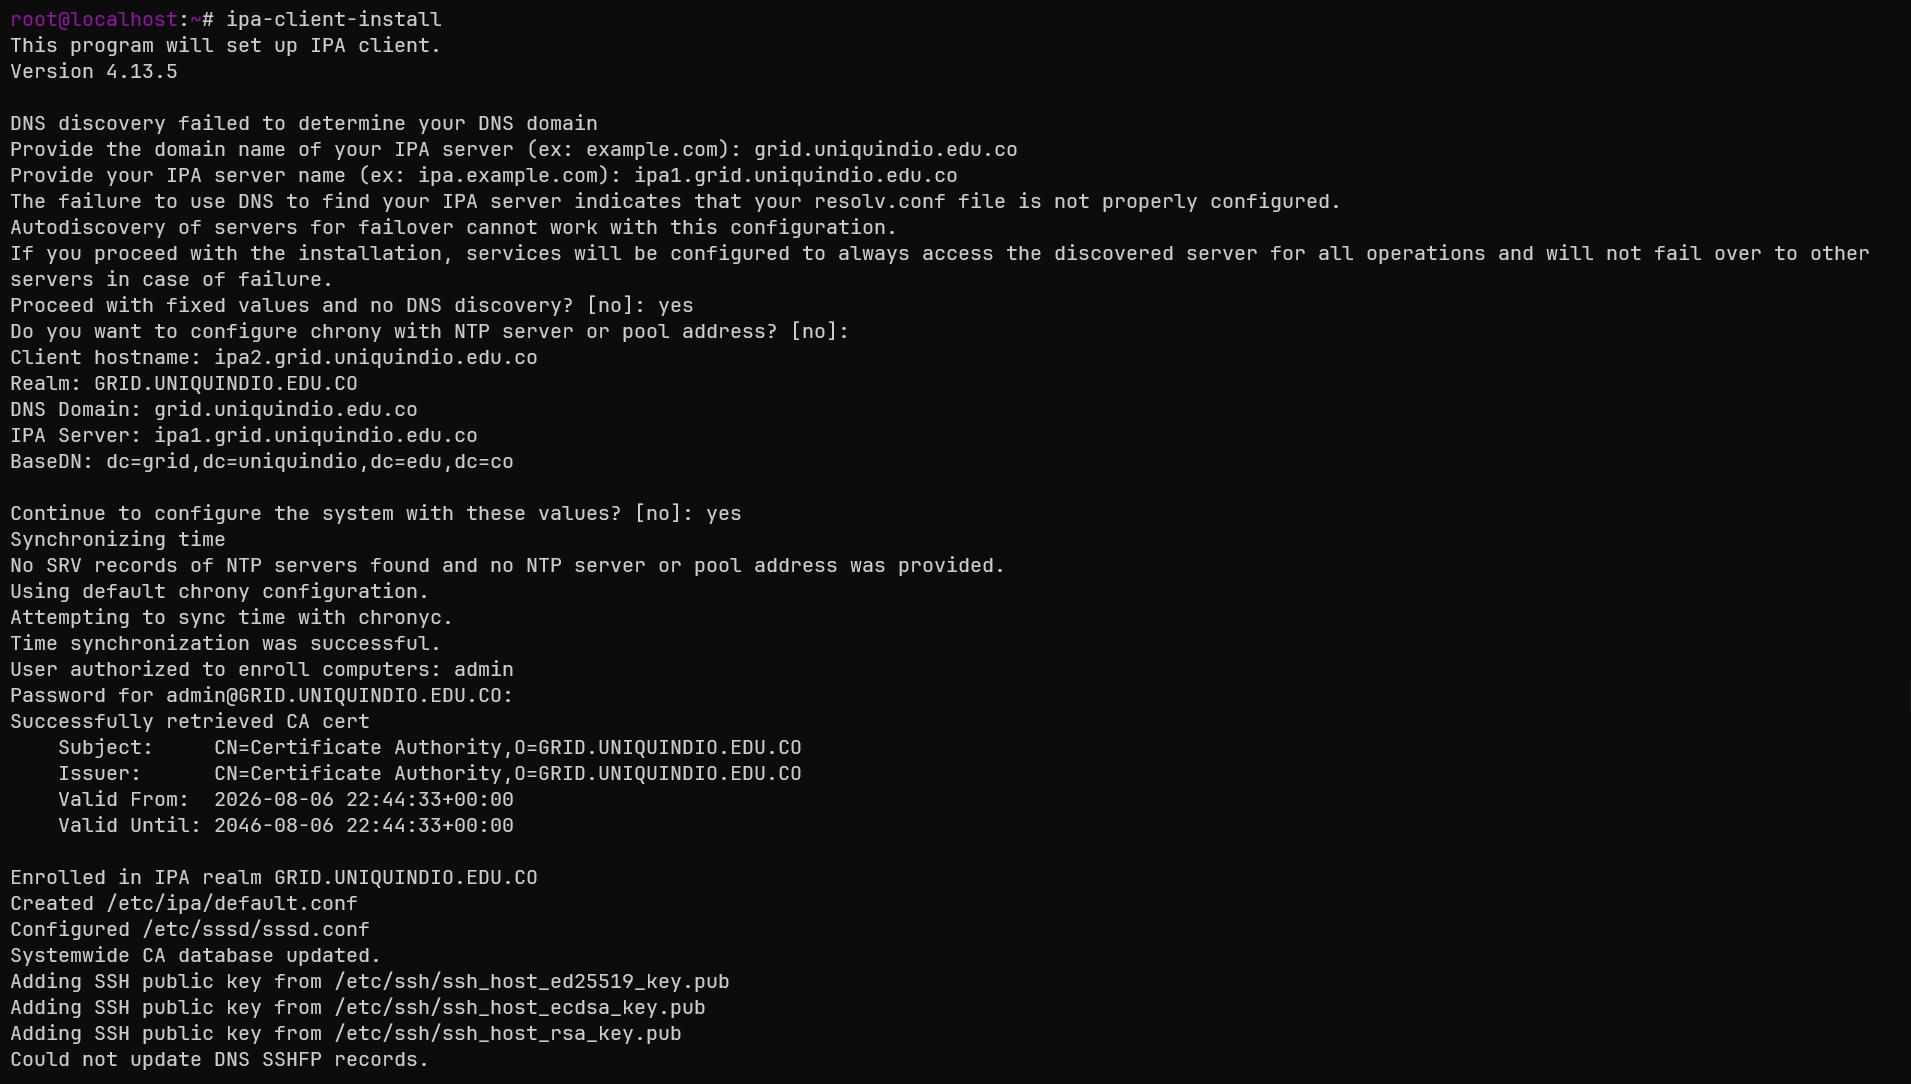
\includegraphics[width=0.8\textwidth]{mainmatter/II-desarrollo-metodologico/implementacion/imagenes/instalacion-cliente-ipa2.png}
	\caption{Instalación del cliente de FreeIPA}
	\label{fig:instalacion-cliente-ipa2}
\end{figure}

Posteriormente, desde el servidor principal se añadió el nuevo equipo al grupo ipaservers, lo que permitió conceder los permisos necesarios para que el sistema pudiera asumir el rol de servidor de réplica. Este procedimiento se muestra en la \autoref{fig:adicion-ipa2-a-ipa1}.

\begin{figure}[H]
	\centering
	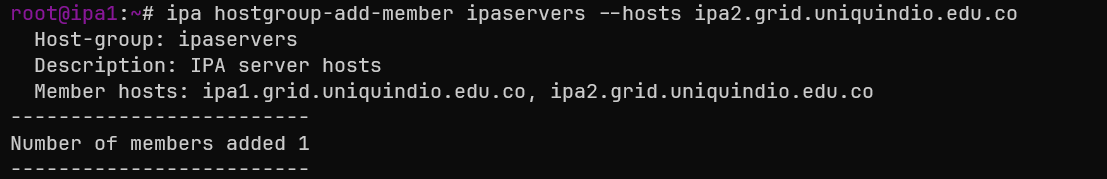
\includegraphics[width=0.8\textwidth]{mainmatter/II-desarrollo-metodologico/implementacion/imagenes/adicion-ipa2-a-ipa1.png}
	\caption{Incorporación del servidor al grupo ipaservers}
	\label{fig:adicion-ipa2-a-ipa1}
\end{figure}

Finalmente, se ejecutó el proceso de promoción del cliente a servidor de réplica, mediante el cual se llevó a cabo la instalación de los componentes necesarios y la sincronización de la información almacenada en el servidor principal. Una vez concluido el procedimiento, se verificó la incorporación del nuevo nodo a la infraestructura, comprobando que este apareciera en el listado de servidores registrados en la plataforma. El proceso de promoción se presenta en la \autoref{fig:promocion-cliente-servidor}, mientras que la \autoref{fig:verificacion-servidor-replica} muestra la verificación de la réplica creada.

\begin{figure}[H]
	\centering
	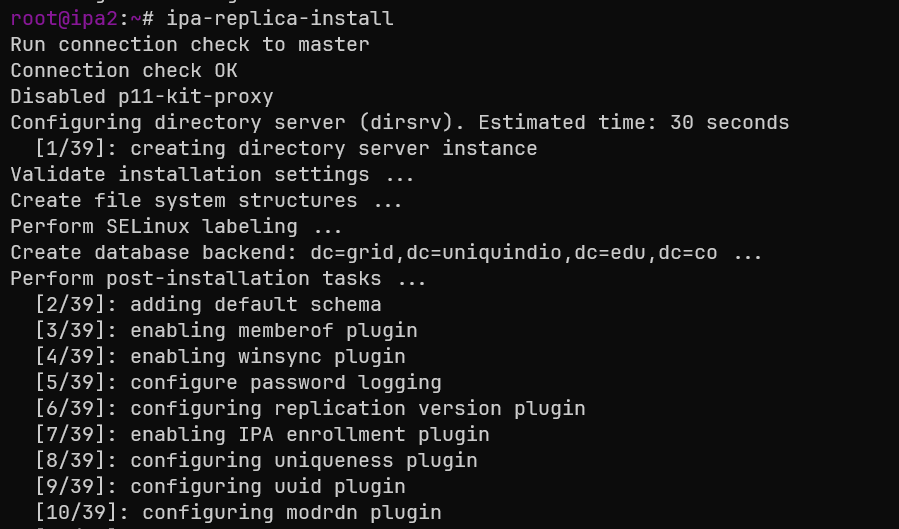
\includegraphics[width=0.8\textwidth]{mainmatter/II-desarrollo-metodologico/implementacion/imagenes/promocion-cliente-servidor.png}
	\caption{Promoción del cliente a servidor de réplica}
	\label{fig:promocion-cliente-servidor}
\end{figure}

\begin{figure}[H]
	\centering
	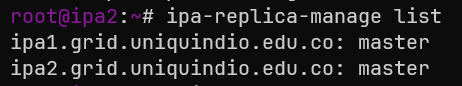
\includegraphics[width=0.8\textwidth]{mainmatter/II-desarrollo-metodologico/implementacion/imagenes/verificacion-servidor-replica.png}
	\caption{Verificación del servidor de réplica}
	\label{fig:verificacion-servidor-replica}
\end{figure}
